\documentclass[tikz]{standalone}
\usepackage{pgfplots}
\pgfplotsset{compat=1.15}
\usepackage{mathrsfs}
\usetikzlibrary{arrows,calc}
\usepackage{tkz-euclide}

\pagestyle{empty}

\definecolor{AngleClr}{rgb}{0,0.39215686274509803,0}
\definecolor{ShapeClr}{rgb}{0.6,0.2,0}

\begin{document}

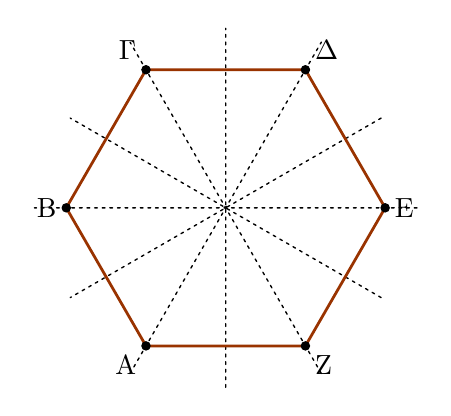
\begin{tikzpicture}[scale=.75]
\tkzSetUpLine[line width=1pt,color=black]
\tkzSetUpPoint[fill=black]

\tkzDefPoints{0/0/P0,2.7/0/P1}

\tkzDefRegPolygon[side,sides=6](P0,P1)

\tkzDefMidPoint(P1,P2) \tkzGetPoint{M1}
\tkzDefMidPoint(P2,P3) \tkzGetPoint{M2}
\tkzDefMidPoint(P3,P4) \tkzGetPoint{M3}
\tkzDefMidPoint(P4,P5) \tkzGetPoint{M4}
\tkzDefMidPoint(P5,P6) \tkzGetPoint{M5}
\tkzDefMidPoint(P6,P1) \tkzGetPoint{M6}

\tkzFillPolygon[fill=white](P1,P2,P3,P4,P5,P6)

\tkzDrawSegments[line width=0.5pt,color=black,dashed,dash pattern=on 1pt off 1.75pt,add=0.1 and 0.1](P1,P4 P2,P5 P3,P6)

\tkzDrawSegments[line width=0.5pt,color=black,dashed,dash pattern=on 1pt off 1.75pt,add=0.15 and 0.15](M1,M4 M2,M5 M3,M6)


\tkzDrawPolygon[color=ShapeClr](P1,P2,P3,P4,P5,P6)
\tkzDrawPoints[size=3](P1,P2,P3,P4,P5,P6)
\tkzLabelPoint[below left](P1){$\rm A$}
\tkzLabelPoint[below right](P2){$\rm Z$}
\tkzLabelPoint[right](P3){$\rm E$}
\tkzLabelPoint[above right](P4){$\rm \Delta$}
\tkzLabelPoint[above left](P5){$\rm \Gamma$}
\tkzLabelPoint[left](P6){$\rm B$}

\end{tikzpicture}

\end{document}
